\documentclass[a4paper]{article}
\usepackage[utf8]{inputenc}
\usepackage[russian,english]{babel}
\usepackage[T2A]{fontenc}
\usepackage[left=10mm, top=20mm, right=18mm, bottom=15mm, footskip=10mm]{geometry}
\usepackage{indentfirst}
\usepackage{amsmath,amssymb}
\usepackage[italicdiff]{physics}
\usepackage{graphicx}
\graphicspath{{images/}}
\DeclareGraphicsExtensions{.pdf,.png,.jpg}
\usepackage{wrapfig}
\usepackage{pgfplots}

\usepackage{caption}
\captionsetup[figure]{name=Рисунок}
\captionsetup[table]{name=Таблица}


\title{\underline{Лабораторная работы 2.2.1}}
\author{Старостин Александр, Б01-401}
\date {3 Марта, 2025 год}


\begin{document}

\maketitle
\newpage

\textbf{Исследование взаимной диффузии газов}

\section{Аннотация}
    \par \textbf{Цель работы:} 1) регистрация зависимости концентрации гелия в воздухе от времени с помощью датчиков теплопроводности при разных начальных давлениях смеси газов; 2) определение коэффициента диффузии по результатам измерений. \\

    \par \textbf{В работе используются:}  измерительная установка; форвакуумный насос; балон с газом  (гелий); манометр; источник питания; магазин сопротивлений; гальванометр; секундомер.

\section{Теоретические сведения}

    \textit{Диффузией}  называют самопроизвольное взаимное проникновение веществ друг в друга происходящее вследствие хаотичного теплового движения молекул. При перемешивании молекул разного сорта говорят о взаимной (или концентрационной) диффузии. В системе, состоящей из двух компонентов a и b (бинарная смесь), плотности потоков частиц в результате взаимной диффузии определяются законом Фика:
    \begin{equation}
        j_a = -D \frac{\partial n_a}{\partial x}, \, j_b = -D \frac{\partial n_b}{\partial x},
    \end{equation}
    где $D$ — \textit{коэффициент взаимной диффузии компонентов}. Знак <<минус>> отражает тот факт, что диффузия идёт в направлении выравнивания концентраций. Равновесие достигается при равномерном распределении вещества по объёму.

    В данной работе исследуется взаимная диффузия гелия и воздуха. Отметим, что давление и температура в системе предполагаются неизменным: $P_0 = (n_{He}+n_{Air})kT = const$, где $n_{He}$  и $n_{Air}$ -- концентрации диффундирующих газов. Поэтому для любых изменений концентраций справедливо $\Delta n_{Air} = -\Delta n_{He}$. Следовательно, достаточно ограничиться описанием диффузии одного из компонентов, например гелия.

    Приведём теоретическую оценку для коэффициента диффузии. В работе концентрация гелия, как правило, мала ($n_{He} \ll n_{Air}$). Кроме того, атомы гелия легче молекул, составляющих воздух ($m_{He} \ll m_{N_2}, m_{O_2}$), значит их средняя тепловая скорость велика по сравнению с остальными частицами. Поэтому перемешивание газов в работе можно приближенно описывать как диффузию примеси лёгких частиц He на практически стационарном фоне воздуха. Коэффициент диффузии в таком приближении равен
    \begin{equation}
        \label{D}
        D = \frac{1}{3} \lambda \langle v \rangle,
    \end{equation}
    где $\lambda = \frac{1}{n\sigma}$ -- длина свободного пробега диффундирующих частиц; $\langle v \rangle = \sqrt{\frac{8kT}{\pi m}}$ -- их средняя тепловая скорость.

    Предпологая, что процесс диффузии будет квазиостационарным, можно показать, что разность концентраций будет убывать по экспоненциальному закону
    \begin{equation}
        \label{Delta_n}
        \Delta n = \Delta n_0 e^{-t / \tau},
    \end{equation}
    где $\tau$ -- характерное время выравнивания концентраций между сосудами, определяемое следующей формулой
    \begin{equation}
        \label{Tau}
        \tau = \frac{1}{D} \frac{V_1V_2}{V_1 + V_2} \frac{L}{S}.
    \end{equation}


\section{Установка}

   Для   исследования   взаимной диффузии газов и измерения коэффициента взаимной диффузии  $D$  используется  два сосуда  объёмами  $V_1$ и $V_2$ ($V_1 \approx V_2$), соединенные трубкой длины $L$ и сечения  $S$. Предполагается, что сосуды заполнены смесью двух газов при одинаковом давлении, но с различной концентрацией компонентов. Вследствие взаимной диффузии, проходящей в   соединительной трубке, концентрации компонентов в сосудах с течением времени выравниваются.

    Для измерения разности  концентраций  в установке применяются датчики теплопроводности. При этом используется тот факт, что теплопроводность смеси $\kappa$ зависит от её состава. В общем случае   зависимость  $\kappa (n)$  довольно   сложна,   однако   при   малой   разности  $\Delta n$ концентраций в сосудах можно ожидать, что разность теплопроводностей будет изменяться прямо пропорционально $\Delta n:$
    \begin{equation*}
        \Delta \kappa = \kappa (n_2) - \kappa (n_1) \approx const \cdot \Delta n.
    \end{equation*}

    Эксперименты показывают, что если доля примеси гелия составляет менее 15\%, отклонение от линейной зависимости не превышает 0,5\%, что для наших целей вполне достаточно.


    При заданной мощности нагревания приращение температуры  проволочки и, следовательно, приращение её сопротивления пропорциональны теплопроводности газа. Для измерения сопротивлений используется мостовая схема, позволяющая определять разность показаний датчиков с высокой точностью. Мост балансируется при заполнении сосудов (и датчиков) одной и той же смесью. При заполнении сосудов смесями различного состава возникает «разбаланc» моста. При незначительном различии в составах смесей показания гальванометра, подсоединённого к диагонали моста, будут пропорциональны разности концентраций примеси: $U\propto\Delta \kappa \propto \Delta n$. В процессе диффузии разность концентраций убывает по закону~(\ref{Delta_n}), и значит по тому же закону изменяются во времени показания гальванометра
    \begin{equation}
        U = U_0 \, e^{-t / \tau},
    \end{equation}
    где $U_0$ -- показание в начальный момент времени. Измеряя экспериментально зависимость $U(t)$, можно получить характерное время процесса $\tau$, откуда по формуле~(\ref{Tau}) определить коэффициент диффузии $D$.

\section{Ход работы}

\subsection{Изучение установки}

Мы изучили установку и зафиксировали значения её параметров:\\

$760 \text{ мм.рт.ст} = 760 \text{ торр} = 101.325 \text{ Па}$.\\

$V_1 = V_2 = (800 \pm 5) \text{ см}^3$,\\

$\frac{L}{S} = (15.0 \pm 0.1) \text{ см}^{-1}$,\\

атмосферное давление в день проведения работы: $P_\text{атм} = 753 \text{ мм.рт.ст} = 101 \text{ дел на манометре}$ (на манометре всего 101 деление), тогда $1 \text{ дел} \approx 7.5 \text{ торр}.$ \\

Доли давлений в колбах после их заполнения воздухом и гелием при выставленном рабочем давлении $P_\text{возд}$: $P_\text{возд} = 1.75 P_\text{раб}$ и $P_\text{гел} = 0.2 P_\text{раб}$.\\

Фотография установки:

\begin{figure}[ht]
        \center{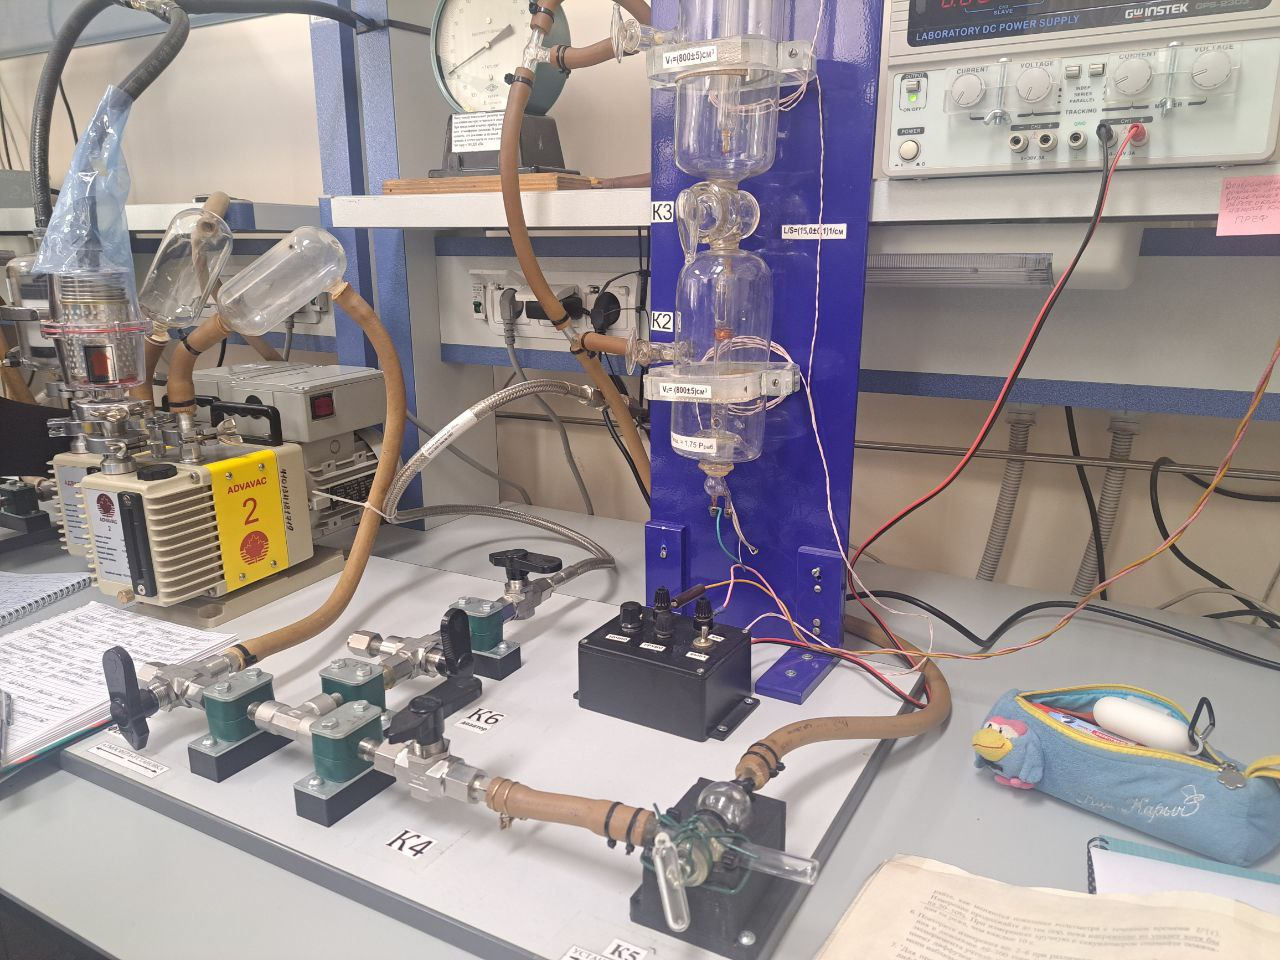
\includegraphics[scale=0.32]{ustanovka}
        \caption{Фотография установки.}
        \label{ustanovka}
\end{figure}

\subsection{Алгоритм проведения диффузии}

Чтобы провести диффузию газов надо выполнить следующие действия:\\

1) открыть все краны, откачать весь воздух из установки с помощью компрессора. \\

2) установить при помощи воздуха из атмосферы рабочее давление в установке, используя показания манометра. \\

3) при помощи моста выровнять напряжение на вольтметре до $\approx 0.0000 \text{ мВ}$; это напряжение настраивается для данного $P_\text{раб}$.  \\

4) открыть все краны, откачать весь воздух из установки с помощью компрессора. \\

5) перекрыть все краны, открыть колбу для гелия, закачать гелий в колбу с помощью манометра до давления $P_\text{гел} = 0.2 P_\text{раб}$; перекрыть колбу с гелием. \\

6) откачать остатки гелия в установке с помощью компрессора. \\

7) открыть колбу для воздуха, из атмосферы запустить в колбу воздух при помощи манометра до давления $P_\text{возд} = 1.75 P_\text{раб}$.  \\

8) открыть колбу с гелием на 30-40 c, чтобы давление в установке успело выровняться; данное действие не испортит результаты измерения диффузии, тк за такое время она не успеет произойти; по манометру определить точное рабочее давление $P_\text{точн}$ ($P_\text{раб}$ \approx $P_\text{точн}$).\\

9) перекрыть колбы с воздухом и гелием; открыть перегордку между колбами, тем самым запустив диффузию газов. \\

10) запустить программу, фиксирующую значения напряжения на вольтметре $U$ от времени $t$ в таблицу и строющую график $U(t)$ для данного $P_\text{раб}$;  продолжать измерения до тех пор, пока напряжение на вольтметре не упадёт на $30-40\%$\\

11) сохранить полученные данные и провести алгоритм уже для другого $P_\text{раб}$.

\subsection{Проведение измерений}

Проведём измерения для 4-ёх рабочих давлений:\\

%----------------------------------------------------
\[P_\text{раб} = 40 \text{ торр}  \]

Отклонение на манометре для $P_\text{раб}$ = $\frac{40}{7.5} \approx 5.5 \text{ дел}$ \\

Отклонение на манометре для $P_\text{возд} = 9.5 \text{ дел}$ \\

Отклонение на манометре для $P_\text{гел} = 1 \text{ дел}$ \\

Отклонение на манометре для $P_\text{точн} = (101 - 96) \text{ дел} = 5 \text{ дел}$

%----------------------------------------------------

%----------------------------------------------------
\[P_\text{раб} = 70 \text{ торр}  \]

Отклонение на манометре для $P_\text{раб}$ = $\frac{70}{7.5} \approx 9 \text{ дел}$ \\

Отклонение на манометре для $P_\text{возд} = 16 \text{ дел}$ \\

Отклонение на манометре для $P_\text{гел} = 2 \text{ дел}$ \\

Отклонение на манометре для $P_\text{точн} = (101 - 92) \text{ дел} = 9 \text{ дел}$

%----------------------------------------------------

%----------------------------------------------------
\[P_\text{раб} = 100 \text{ торр}  \]

Отклонение на манометре для $P_\text{раб}$ = $\frac{70}{7.5} \approx 13 \text{ дел}$ \\

Отклонение на манометре для $P_\text{возд} = 23 \text{ дел}$ \\

Отклонение на манометре для $P_\text{гел} = 3 \text{ дел}$ \\

Отклонение на манометре для $P_\text{точн} = (101 - 87.5) \text{ дел} = 13.5 \text{ дел}$

%----------------------------------------------------

%----------------------------------------------------
\[P_\text{раб} = 130 \text{ торр}  \]

Отклонение на манометре для $P_\text{раб}$ = $\frac{130}{7.5} \approx 17 \text{ дел}$ \\

Отклонение на манометре для $P_\text{возд} = 30 \text{ дел}$ \\

Отклонение на манометре для $P_\text{гел} = 3.5 \text{ дел}$ \\

Отклонение на манометре для $P_\text{точн} = (101 - 84) \text{ дел} = 17 \text{ дел}$

%----------------------------------------------------

\subsection{Обработка результатов}

Если верна формула (5), то и верна формула (3). Тогда обработаем значения, полученные для каждого $P_\text{раб}$, при помощи графиков ln$U$ от $t$ (должны быть прямые). \\

Так же для нашей установки из (4) получаем:

\begin{equation}
        \label{D_new}
        D = \frac{V}{2\tau} \frac{L}{S}.
\end{equation}

%----------------------------------------------------
\[P_\text{раб} = 40 \text{ торр}  \]

По данным в полученной таблице построим график ln$U$ от $t$:

\begin{figure}[ht]
        \center{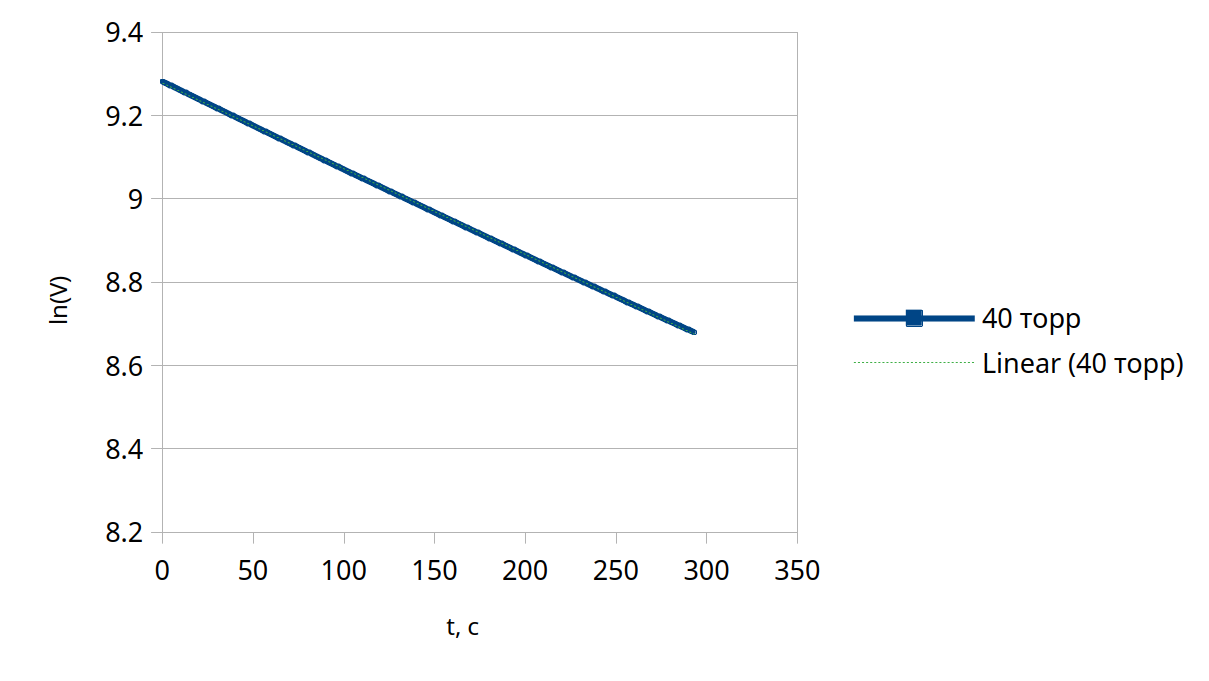
\includegraphics[scale=0.45]{40}
        \caption{график ln$U$ от $t$ при 40 торрах}
        \label{ustanovka}
\end{figure}

По МНК проведём наилучшую прямую $y = kx + b$. \\

Тогда $k = -\frac{1}{\tau} = \frac{<xy> - <x><y>}{<x^2> - <x>^2} = -0.002056 \text{ с}^{-1}$.\\

И $\sigma_k = \sqrt{\frac{1}{295}} \sqrt{\frac{<y^2> - <y>^2}{<x^2> - <x>^2} - k^2} = 0.0002 \text{ с}^{-1}$.\\

Тогда $k = (-0.0021 \pm 0.0002) \text{ с}^{-1}$.  \\

Получем: $D = 12.6 \frac{\text{ см}^2}{\text{с}}$. \\

%----------------------------------------------------
%\newpage
%----------------------------------------------------
\[P_\text{раб} = 70 \text{ торр}  \]

По данным в полученной таблице построим график ln$U$ от $t$:

\begin{figure}[ht]
        \center{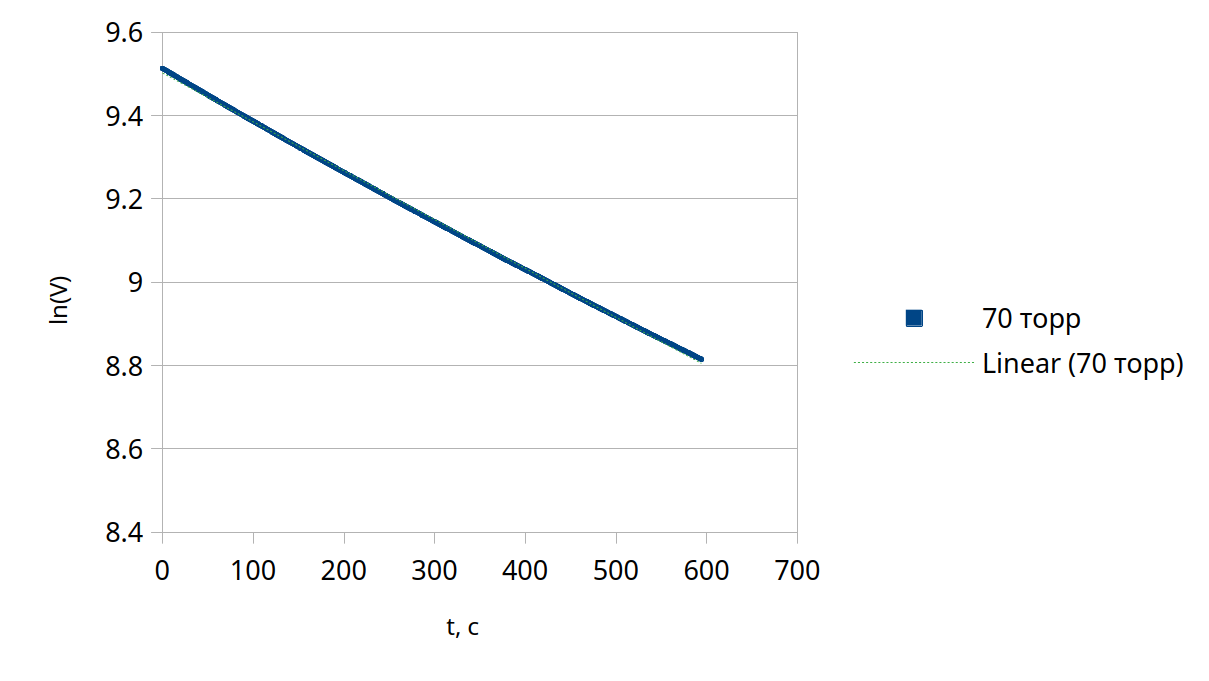
\includegraphics[scale=0.45]{70}
        \caption{график ln$U$ от $t$ при 70 торрах}
        \label{ustanovka}
\end{figure}

По МНК проведём наилучшую прямую $y = kx + b$. \\

Тогда $k = -\frac{1}{\tau} = \frac{<xy> - <x><y>}{<x^2> - <x>^2} = -0.001173  \text{ с}^{-1}$.\\

И $\sigma_k = \sqrt{\frac{1}{596}} \sqrt{\frac{<y^2> - <y>^2}{<x^2> - <x>^2} - k^2} = 0.0001 \text{ с}^{-1}$.\\

Тогда $k = (-0.0012 \pm 0.0001) \text{ с}^{-1}$.  \\

Получем: $D = 7.2 \frac{\text{ см}^2}{\text{с}}$.

%----------------------------------------------------
\newpage
%----------------------------------------------------
\[P_\text{раб} = 100 \text{ торр}  \]

По данным в полученной таблице построим график ln$U$ от $t$:

\begin{figure}[ht]
        \center{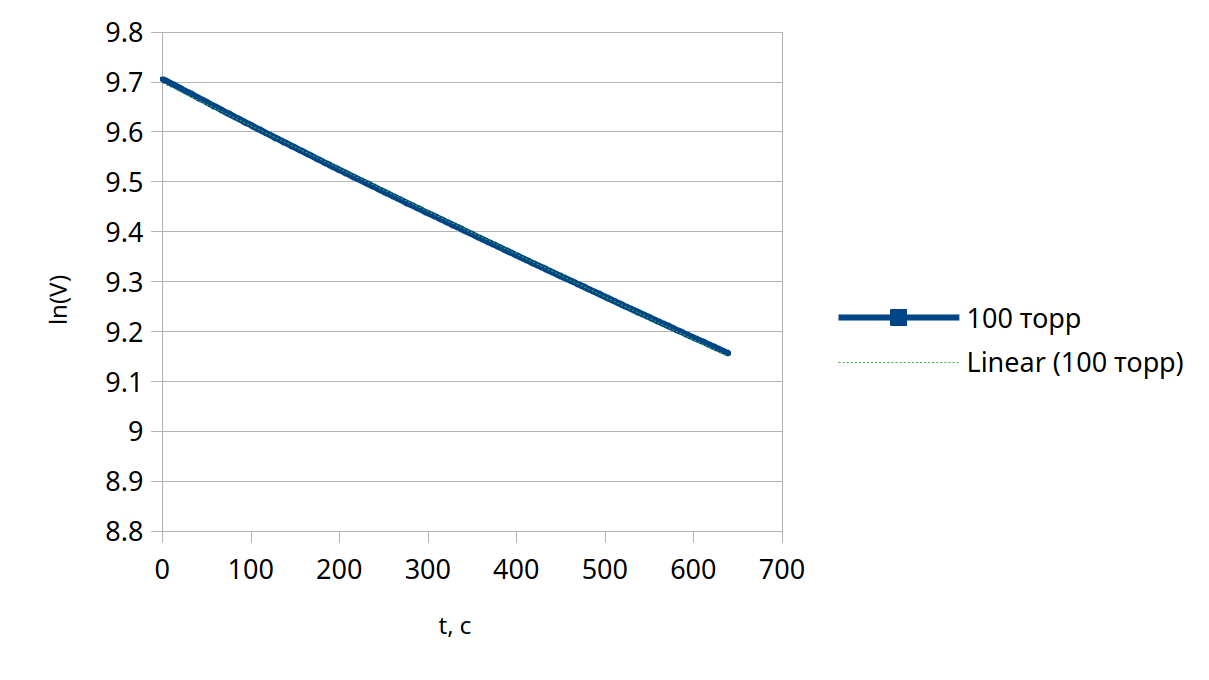
\includegraphics[scale=0.45]{100}
        \caption{график ln$U$ от $t$ при 100 торрах}
        \label{ustanovka}
\end{figure}

По МНК проведём наилучшую $y = kx + b$. \\

Тогда $k = -\frac{1}{\tau} = \frac{<xy> - <x><y>}{<x^2> - <x>^2} =  -0.000857   \text{ с}^{-1}$.\\

И $\sigma_k = \sqrt{\frac{1}{641}} \sqrt{\frac{<y^2> - <y>^2}{<x^2> - <x>^2} - k^2} = 0.00009 \text{ с}^{-1}$.\\

Тогда $k = (-0.00086 \pm 0.00009) \text{ с}^{-1}$. \\

Получем: $D = 5.2 \frac{\text{ см}^2}{\text{с}}$.

%----------------------------------------------------
\newpage
%----------------------------------------------------
\[P_\text{раб} = 130 \text{ торр}  \]

По данным в полученной таблице построим график ln$U$ от $t$:

\begin{figure}[ht]
        \center{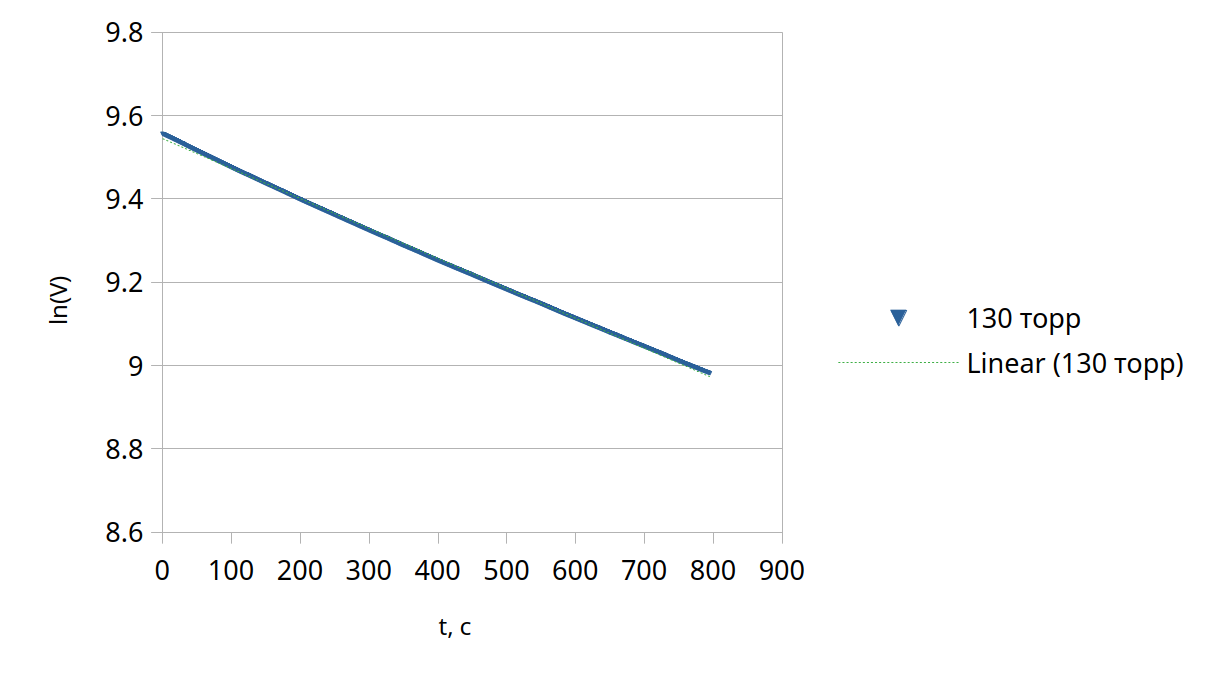
\includegraphics[scale=0.45]{130}
        \caption{график ln$U$ от $t$ при 130 торрах}
        \label{ustanovka}
\end{figure}

По МНК проведём наилучшую прямую $y = kx + b$. \\

Тогда $k = -\frac{1}{\tau} = \frac{<xy> - <x><y>}{<x^2> - <x>^2} =  -0.000719   \text{ с}^{-1}$.\\

И $\sigma_k = \sqrt{\frac{1}{641}} \sqrt{\frac{<y^2> - <y>^2}{<x^2> - <x>^2} - k^2} = 0.00007 \text{ с}^{-1}$.\\

Тогда $k = (-0.00072 \pm 0.00007) \text{ с}^{-1}$. \\

Получем: $D = 4.3 \frac{\text{ см}^2}{\text{с}}$.  \\

%----------------------------------------------------

В каждом случае погрешность $\sigma_D = D\sqrt{(\frac{\sigma_k}{k})^2 + (\frac{\sigma_{L/S}}{L/S})^2 + (\frac{\sigma_V}{V})^2 + (\frac{\sigma_U}{U_0ln\frac{1}{2}})^2}$

\subsection{Зависимость $D$ от $P$}

Постоим график зависмости $D$ от $\frac{1}{P}$

\newpage

\begin{figure}[ht]
        \center{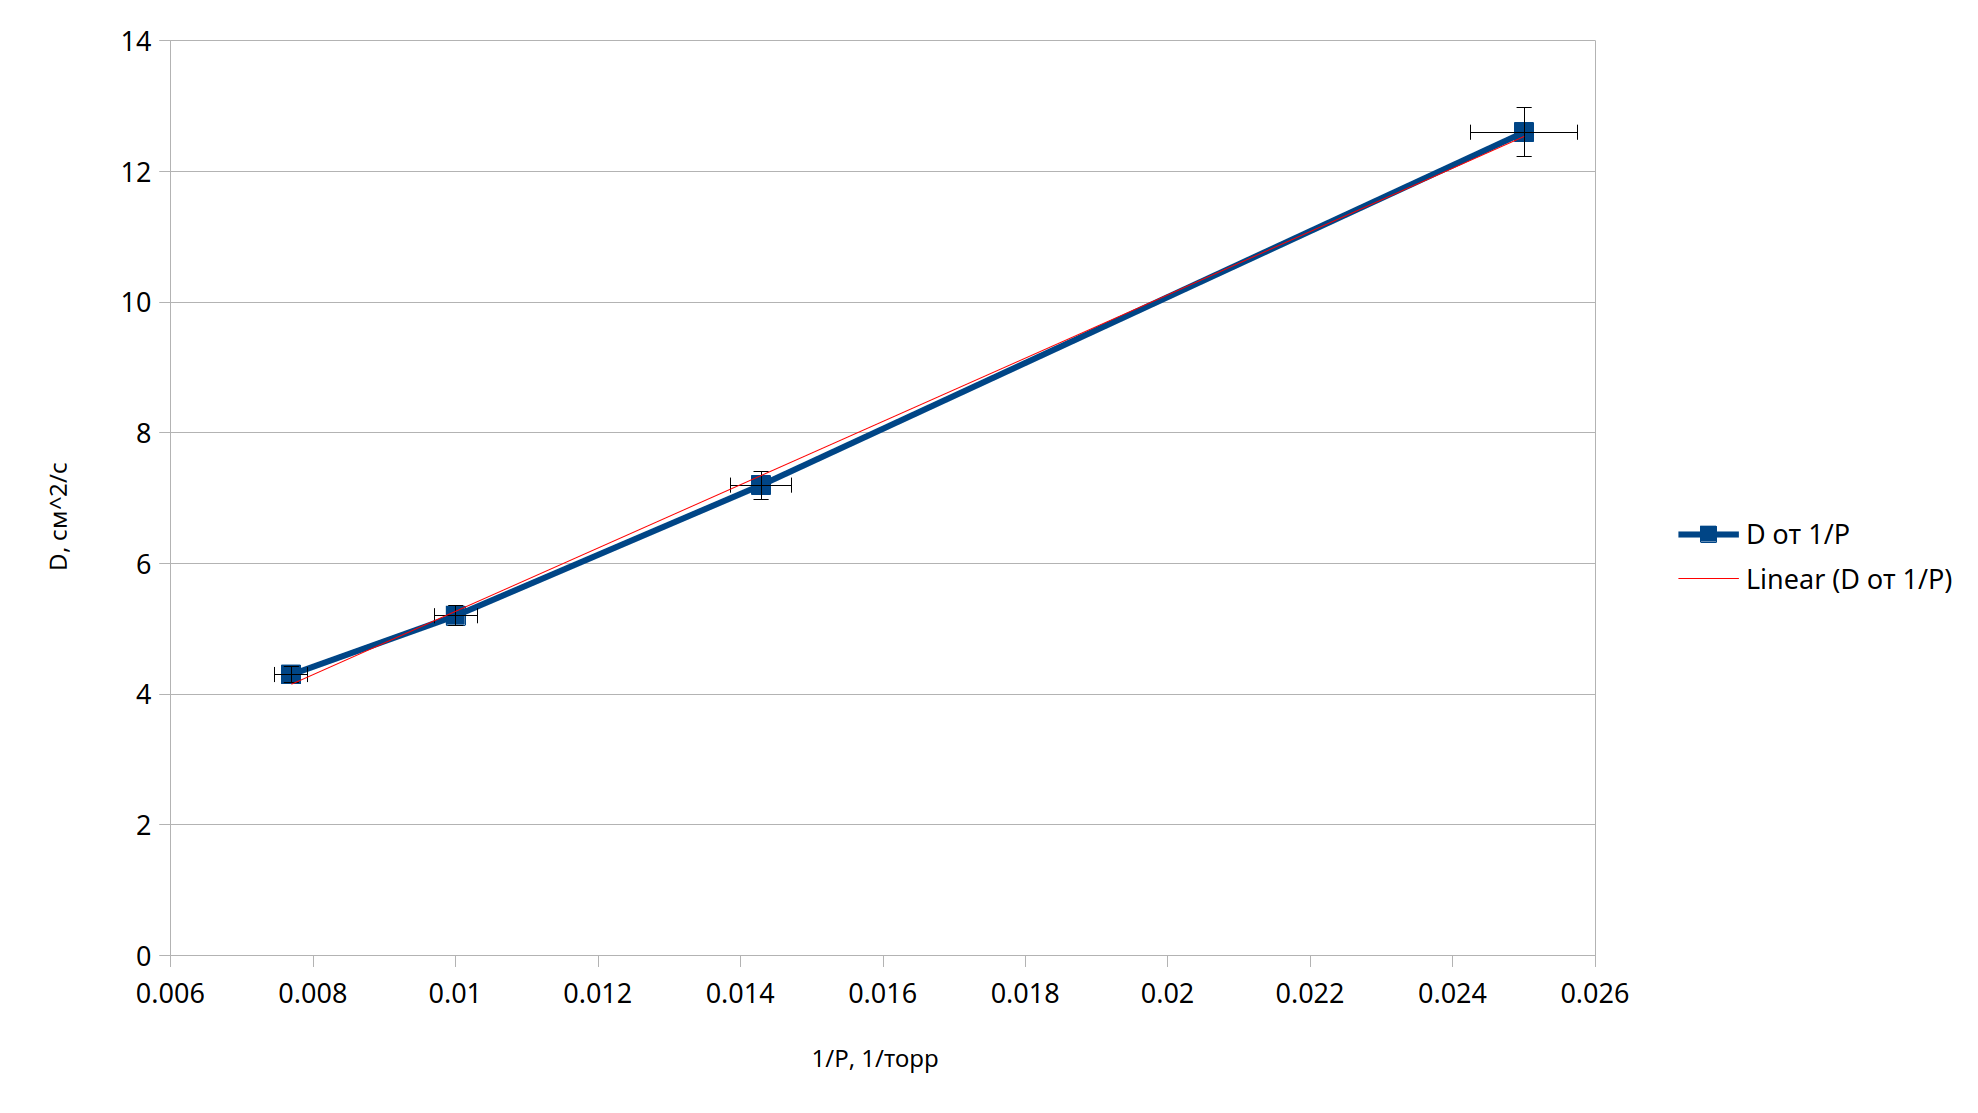
\includegraphics[scale=0.27]{D_and_1⁄P}
        \caption{график зависмости $D$ от $\frac{1}{P}$}
        \label{ustanovka}
\end{figure}

Как мы видим, график линейный. \\

По МНК проведём наилучшую прямую $y = kx + b$. \\ %f(x) = 484.46076 x + 0.424096

Тогда $k = 484.46 \frac{\text{см}^2}{\text{с}*\text{торр}}$ и $b = 0.42 \frac{\text{ см}^2}{\text{с}}$.

При этом $\sigma_k = \sqrt{\frac{1}{4}} \sqrt{\frac{<y^2> - <y>^2}{<x^2> - <x>^2} - k^2} = 48.4 \frac{\text{см}^2}{\text{с}*\text{торр}}$. \\

А $\sigma_b = \sigma_k\sqrt{<x^2> - <x>^2} = 0.03 \frac{\text{ см}^2}{\text{с}}$. \\

При нашем $P_\text{атм} = 753 \text{ торр}$ получаем, что $D_\text{атм} = 1.06 \frac{\text{ см}^2}{\text{с}}$

И $\sigma_D =\sqrt{ D_\text{атм}^2 ((\frac{\sigma_k}{k})^2 + (\frac{\sigma_P}{P})^2)^2 +  \sigma_b^2} = 0.1 \frac{\text{ см}^2}{\text{с}}$

\section{Вывод}

Мы регистрировали зависимость концентрации гелия в воздухе от времени с помощью датчиков при разных начальных давлениях смеси газов,  вычислили коэффициенты диффузии по результатам измерений и коэффициент диффузии при атмосферном давлении, который совпал с табличным занчением.

\end{document}












